\documentclass[ngerman, fleqn, DIV=15, headinclude]{scrartcl}

\usepackage[color]{header}

\hypersetup{
    pdftitle=NetSec Sheet 4
}


\theoremstyle{definition}
\newtheorem{exercise}{Task}

\usepackage{tikz}
\usetikzlibrary{arrows.meta}

%\subject{}
\title{}
%\subtitle{}
\author{
    Timm Behner \\ \small{\href{mailto:behner@cs.uni-bonn.de}{behner@cs.uni-bonn.de}} \and
    Christopher Kannen \\ \small{\href{mailto:ckannen@uni-bonn.de}{ckannen@uni-bonn.de}}
}

\begin{document}

\maketitle

%\newpage
%\tableofcontents
%\newpage

\setcounter{exercise}{1}

\begin{exercise}
    The involved hosts are hellgate (10.0.0.1), white (10.0.0.5) and orange
    (10.0.0.10).
    \begin{figure}[H]
        \centering
        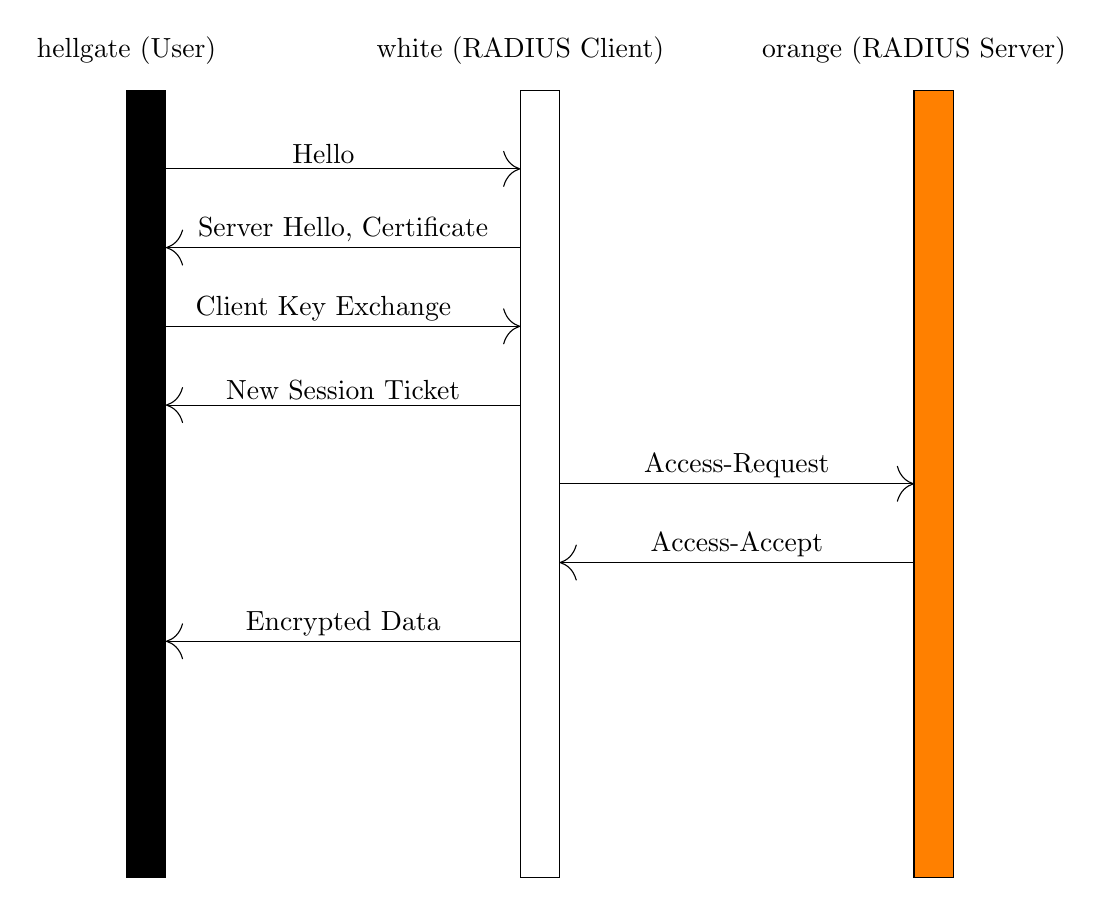
\begin{tikzpicture}
            \foreach \x/\text in {0/hellgate (User), 5/white (RADIUS Client),
            10/orange (RADIUS Server)}
            {
                \node at (\x,5.5) {\text};
            }
            \draw[fill=black] (0  ,-5) rectangle (0.5,5);
            \draw[fill=white] (5  ,-5) rectangle (5.5,5);
            \draw[fill=orange] (10,-5) rectangle (10.5,5);
            \draw[-{>[scale=2.5]}] (0,4) -- node[yshift=-5,label=Hello] {} (5,4);
            \draw[-{>[scale=2.5]}] (5,3) -- node[yshift=-5,label={Server Hello, Certificate}] {} (0.5,3);
            \draw[-{>[scale=2.5]}] (0,2) -- node[yshift=-5,label=Client Key Exchange] {} (5,2);
            \draw[-{>[scale=2.5]}] (5,1) -- node[yshift=-5,label={New Session Ticket}] {} (0.5,1);
            \draw[-{>[scale=2.5]}] (5.5,0) -- node[yshift=-5,label={Access-Request}] {} (10,0);
            \draw[-{>[scale=2.5]}] (10,-1) -- node[yshift=-5,label={Access-Accept}] {} (5.5,-1);
            \draw[-{>[scale=2.5]}] (5,-2) -- node[yshift=-5,label={Encrypted Data}] {} (0.5,-2);
        \end{tikzpicture}
    \end{figure}
\end{exercise}

\begin{exercise}
\end{exercise}

\begin{exercise}\hfill

    \begin{enumerate}[a)]
        \item \hfill

            \begin{itemize}
                \item \textbf{Authentication by finger print}

                    Use your finger print instead of a password. This method
                    is e.g. used by smartphones and Laptops such as iPhone 6.
                    A big advantage is that you can't forget your finger print
                    and the authentication can be much faster than typing in a
                    password.  A disadvantage is that with currently used
                    sensors, this method can be hacked very easily by printing
                    the finger print line on a piece of paper and let the
                    sensor scan this paper.
        
                \item \textbf{Authentication by swipe card / chip card}

                    This method is used by credit and debit cards. Mostly together with
                    a PIN or signature, but for smaller amounts there is also the
                    option to use this method even without a second verification.  An
                    advantage is that this method is very fast and easy to use.  A
                    disadvantage is that if the card gets stolen, the thief can use it
                    to get money from your bank account, because the one who has the
                    card card (even if it is not the owner) has access to the account.
            
                \item \textbf{Authentication by MAC-Address}

                    This is used in wireless networks, most common additionally to a
                    password, to allow computers to join the network.  It gives a
                    certain amount of security, although it can be changed by hackers,
                    the MAC address of a network device is usually fixed, so only
                    registered devices can access the network.  A disadvantage is that
                    the administrative costs raise, since every device has to be set up
                    in the back end.

            \end{itemize}
        \item Authentication by MAC-Address is also an example for a two-factor authentication, when a common password is used besides the MAC address comparison.
                This raises the security of networks, which is a plus. The disadvantage is the higher costs mentioned in a)
    \end{enumerate}
\end{exercise}

\begin{exercise}\hfill

    \begin{enumerate}[a)]
        \item \verb$task_5.py$ is an implementation of CBC with ROT-128 to
            produce a MAC. For an example output with the MAC of the exercise
            sheet see \verb$task_5_pdfmac.txt$
        \item For ECB and CTR the MAC would consist of $C_1, \cdots , C_n$
            since every single $C_i$ would be needed to check the integrity of
            the document. This would lead either to a very large MAC or to a
            very short length of every $C_i$ which would lead to more
            collisions and thus would be a weaker MAC.

            With CBC only the last $C_n$ is needed to check the integrity of
            the document since a change in any $P_1, \cdots, P_n$ would lead to
            a different output. Since only the last $C_n$ chunk is needed this
            can be large enough to make collisions very unlikely.
    \end{enumerate}
\end{exercise}
\end{document}

% vim: spell spelllang=en tw=79
